% 多普勒效应(一维匀速)

\pentry{平面波\upref{PWave}}

\textbf{多普勒效应(Doppler effect)}是讨论, 当机械波的波源和(或)接收者相对于波的介质运动时, 发射的频率和接收到的频率之间有何关联. 本文不讨论相对论效应, 即假设波速远小于真空中的光速, 另外本文只讨论波源和接收者沿同一直线匀速运动的情况.

\begin{figure}[ht]
\centering
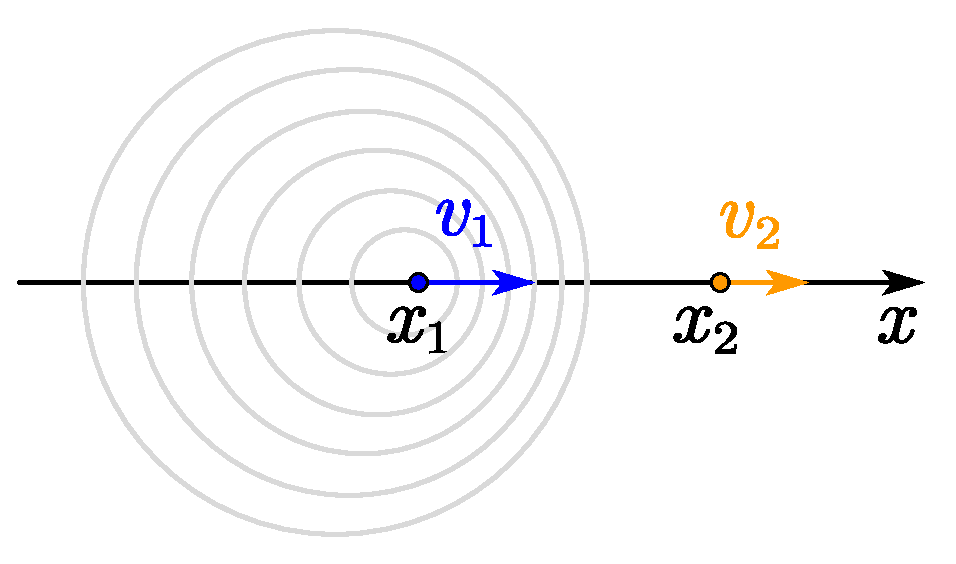
\includegraphics[width=6cm]{./figures/Dople1_1.pdf}
\caption{多普勒效应} \label{Dople1_fig1}
\end{figure}

\begin{example}{}
生活中一种常见的多普勒效应是, 一辆疾驰的车一边鸣笛一边驶过行人, 人听到的音调就会先高后低. 这是因为, 车经过人之前不断靠近人, 经过人后再不断远离人. 可见多普勒效应和运动的速度有关.
\end{example}

在分析多普勒效应时, 一种方便的做法是选取介质为参考系, 例如有均匀的风时, 参考系随风运动. 假设介质处处均匀且静止, 波在介质中传播的速度(\textbf{波速}) $v$ 处处相等, 且与方向无关(\textbf{各向同性}).

令\autoref{Dople1_fig1} 中波源甲运动方程, 即位置关于时间的函数为 $x_1(t)$, 对时间求导得到速度 $v_1(t) = \dot{x}_1(t)$. 同理, 接收者乙位置和速度分别为 $x_2(t)$ 和 $v_2(t)$. 注意两个点的速度都是向右运动为正, 向左运动为负. 令波源的频率为 $f_1$, 接收者收到的频率为 $f_2$. 当两点分别以小于波速的速度($\abs{v_1}, \abs{v_2} < v$)匀速运动时, 有
\begin{equation}\label{Dople1_eq1}
\frac{f_2}{f_1} = \frac{v \mp v_2}{v \mp v_1}
\end{equation}
该式当 $x_1 < x_2$ 时上式取负号, 当 $x_2 < x_1$ 时上式取正号. 由该式可以发现, 波源和接受者是对称的, 即如果乙作为波源发射 $f_2$ 的波, 那么甲接收到的频率同样是 $f_1$.

\begin{exercise}{}
在一条长直马路上, 风速为 $10\Si{m/s}$, 一个单车以 $5\Si{m/s}$ 向顺风而行, 迎面驶来一辆摩托车, 速度为 $20\Si{m/s}$. 若摩托车一直以 $600\Si{Hz}$ 的频率鸣喇叭, 声速为 $340\Si{m/s}$, 求摩托车经过单车前后骑单车的人听到的频率.

令风马路为 $x$ 轴, 风向为正方向, 在风的参考系中, 摩托车速度为
\begin{equation}
v_1 = -20 - 10 = -30(\Si{m/s})
\end{equation}
单车速度为
\begin{equation}
v_2 = 5 - 10 = -5\Si{m/s}
\end{equation}
另外 $v = 340\Si{m/s}$, 相遇以前 $x_2 < x_1$, 所以
\begin{equation}
f_2 = \frac{v + v_2}{v + v_1} f_1 = 648.4\Si{Hz}
\end{equation}
相遇以后 $x_1 < x_2$, 所以
\begin{equation}
f_2 = \frac{v - v_2}{v - v_1} f_1 = 559.5\Si{Hz}
\end{equation}
\end{exercise}
注意我们必须在风的参考系中计算, 否则得不到正确的结果.

\subsection{推导}
本质上, 多普勒效应可以等效为追及问题, 可以想象甲以一定的频率 $f_1$ 向乙发射速度为 $u$ 的子弹, 子弹的位置对应波峰的位置, 两个相邻子弹之间的间距对应波长. 若甲乙相对介质静止不动或者以相同的速度运动, 则乙接收到子弹的频率和甲发射的频率是一样的, 但若甲乙不断靠近, 则接收子弹的频率就会更高, 若不断远离, 则接受的频率就更低.

以 $x_1 < x_2$ 为例, 假设波源在某时刻在 $x_{10}$ 位置向右发射一枚子弹, 经过周期 $T_1 = 1/f_1$ 后又发射第二枚时, 第一枚的位置为 $x_{10} + vT_1$, 而此时波源的位置(也就是第二枚子弹的位置)为 $x_{10} + v_1 T_1$. 所以两枚子弹相距(也就是波长)为
\begin{equation}
\lambda = (v - v_1)T_1
\end{equation}
同理, 接收者收到这两枚子弹的时间间隔为
\begin{equation}
T_2 = \lambda/ (v - v_2)
\end{equation}
以上两式消去 $\lambda$, 有
\begin{equation}
\frac{f_2}{f_1} = \frac{T_1}{T_2} = \frac{v - v_2}{v - v_1}
\end{equation}
这样就得到了\autoref{Dople1_eq1}. $x_2 < x_1$ 的推导同理可得.
